
\documentclass[12pt]{article}
\usepackage{amsmath, amssymb, amsfonts, amsthm}
\usepackage{graphicx}
\usepackage{bbold}
\begin{document}

\section*{Notes: Balancing on elastic contacts}


\subsection*{Elastic contact Model}

The robot model is 2d plan Y-Z. It as 4DoF consisting of two prismatic knees and two rotational hips.
It has two elastic point contact feet with stiffness $K_x$ and $K_y$.
The inertias and kinematics parameters are similar to the HRP2 robot model. 
\begin{figure}[!h]
\centering
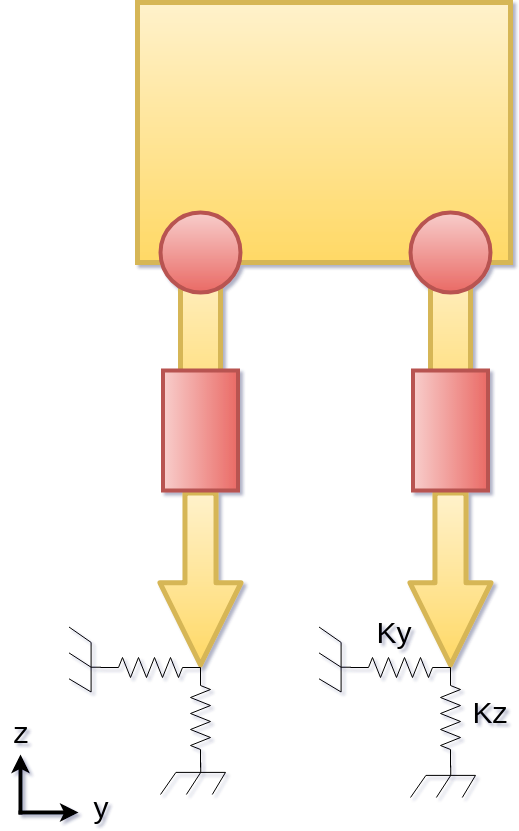
\includegraphics[scale=0.3]{fig/simple_model.png} 
\caption{Simple 4DoF - 2d robot model}
\label{Tux}
\end{figure}

\subsection*{Inverse dynamic contoller}
We want to stabilise the center of mass of the robot. Actuators can apply torques (or forces in the case of the knees) noted $\tau$. Feet position $p_l$, $p_r$ are linked to the contact forces $f_l$, $f_r$ by the elastic spring relationship 
$$ f_i = K_i p_i$$
where $i \in [l,r]$, and $K_i = diag(K_y,K_z)$

Center of mass acceleration is linked to the contact forces by Newton equation
$$\sum f_i +mg= m\ddot{c}$$
We note 
$f = \begin{pmatrix} 
f_l &f_r 
\end{pmatrix}^T
$
and 
$X = \begin{pmatrix} 
\mathbb{1}_2 & \mathbb{1}_2
\end{pmatrix}$, 
so that 
$$X f +mg= m\ddot{c}$$

Since we control the joint torques, equivalent to articular accelerations, we differentiate this equation to express the effect of feet acceleration on the snap of the center of mass.
$$X \ddot{f}= m\ddddot{c}$$
Using the elastic contact relationship,
$$X K\ddot{p}= m\ddddot{c}$$
with $K = diag(K_l,K_r)$ and $p = \begin{pmatrix} p_l & p_r \end{pmatrix}^T$.

$$\ddot{p}=J_p\dot v + \dot J v$$

where $J_p = \begin{pmatrix} J_l & J_r \end{pmatrix}^T$ is the Jacobian of the contact points and $v$ is the articular velocity vector.

Finally, an inverse dynamic controller can choose $\dot v$ in order to drive the CoM dynamic throw the control input $\ddddot{c}^d$

The CoM task cost beeing 

$$\| X K J_p \dot{v} - \ddddot{c}^d-X K \dot{J_p} v\|^2$$

There is a first problem with this task because the angular Momentum is imposed but not regulated. Even with a posture task, there could be internal forces that satisfies the CoM task, but will lead to a diverging Angular Momentum.

Applying the same methodology, we derive the 4th order dynamic linking feet accelerations to Angular Momentum.
Euler's second law gives the relationship between the rate of change of angular momentum $l$ and the CoM.

$$ \dot{l} = \sum (p_i - c) \times f_i $$
$$ \dot{l} = \sum [(p_{iy}-c_{iy})f_{iz} - (p_{iz}-c_{iz})f_{iy}]$$
$$ \ddot{l} = \sum [(\dot{p_{iy}}-\dot{c_{iy}})f_{iz} + (p_{iy}-c_{iy})\dot{f_{iz}} 
                  - (\dot{p_{iz}}-\dot{c_{iz}})f_{iy} - (p_{iz}-c_{iz})\dot{f_{iy}}]$$

$$ \dddot{l} = \sum [(\ddot{p_{iy}}-\ddot{c_{iy}})     f_{iz} + (\dot{p_{iy}}-\dot{c_{iy}}) \dot{f_{iz}}  
                     +(\dot{p_{iy}}- \dot{c_{iy}})\dot{f_{iz}} +     (p_{iy}-      c_{iy}) \ddot{f_{iz}}$$
$$                  -(\ddot{p_{iz}}-\ddot{c_{iz}})     f_{iy} - (\dot{p_{iz}}-\dot{c_{iz}}) \dot{f_{iy}} 
                     -(\dot{p_{iz}}- \dot{c_{iz}})\dot{f_{iy}} -     (p_{iz}-      c_{iz}) \ddot{f_{iy}}]$$
knowing that $\ddot{p_{iy}} = K_y^{-1} \ddot{f_y}$ and $\ddot{p_{iz}} = K_z^{-1} \ddot{f_iz}$, we can write $\dddot{l}$ as a linear function of $\ddot f$:

$$\dddot{l} = N_l + X_l \ddot f$$
where 
$$X_l= \begin{pmatrix} 
        +K_y^{-1}f_{lz} - (p_{lz} - c_z) \\
        -K_z^{-1}f_{ly} + (p_{ly} - c_y) \\
        +K_y^{-1}f_{rz} - (p_{rz} - c_z) \\
        -K_z^{-1}f_{ry} + (p_{ry} - c_y) 
\end{pmatrix}$$
and 
$$N_l= f_{ly}\dot{c_{iz}} - f_{lz}\dot{c_{iy}} + 2[(\dot{p_{ly}}-dcy)\dot{f_{lz}} - (\dot{p_{lz}}-dcz)\dot{f_{ly}}]$$

Finally, 
$$\dddot{l} = N_l + X_l K \ddot p$$
The Angular Momentum task is then:
$$\| X_l K J_p \dot{v} - \dddot{l}^d- N_l - X_l K \dot{J_p} v\|^2$$

Stacking CoM and Angular Momentum tasks, we get the full 4th order centroidal task:


$$\| \begin{pmatrix}  X_c \\ X_l \end{pmatrix} K J_p \dot{v} - \begin{pmatrix}  \ddddot{c}^d \\ \dddot{l}^d \end{pmatrix}- \begin{pmatrix}  0 \\ N_l \end{pmatrix} - \begin{pmatrix}  X_c \\ X_l \end{pmatrix} K \dot{J_p} v\|^2$$


\subsection*{Linear Feedback Regulator}
As seen before, the inverse dynamic formulation is capable of controlling $\dddot{l}$ and $\ddddot{c}$.
So the system to control is a pure 4th order integrator.

We note x the centroidal state composed of ${c, l^\Sigma}$

$l^\Sigma$ should be the integral of the angular momentum but this is not a measurable quantity. We choose to approximate this quantity by $l^\Sigma = i \theta$ where $i$ is the robot inertia, and theta the base orientation representing the majority of the robot weight

The control input is then $\ddddot{x}^d= \begin{pmatrix}  \ddddot{c}^d \\ \dddot{l}^d \end{pmatrix}$

We can apply a linear feedback as control input:

$$\ddddot{x}^d = K_p(x^* - x) + K_v(\dot{x}^*-\dot{x})+ K_a(\ddot{x}^*-\ddot{x})+K_j(\dddot{x}^*-\dddot{x})$$

\begin{verbatim}
sigma_c = 0.0005 
sigma_dc = 0.005
sigma_ddc = 0.01
sigma_dddc = 10.

kf_sigma_c = sigma_c
kf_sigma_dc = sigma_dc
kf_sigma_ddc = sigma_ddc
kf_sigma_process_noise = 1e4
\end{verbatim}


\begin{figure}[!h]
\centering
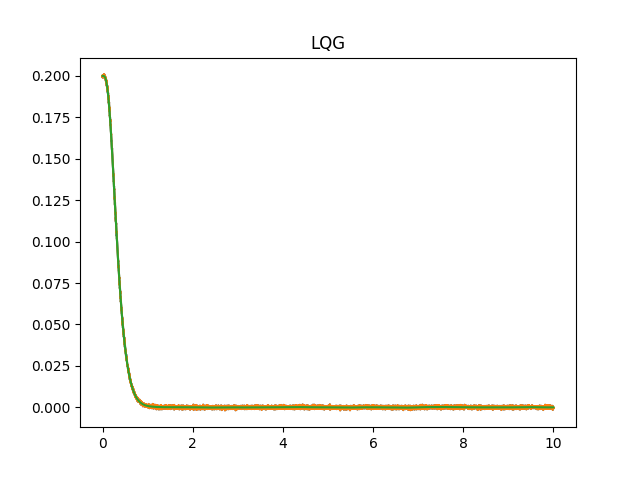
\includegraphics[scale=1]{fig/LQG_regulation.png} 
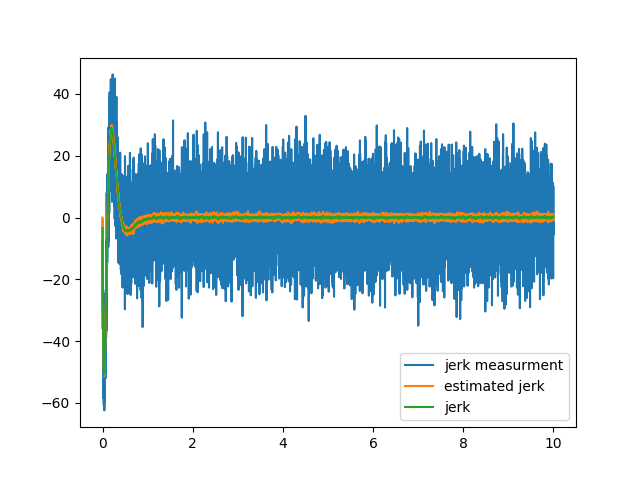
\includegraphics[scale=1]{fig/LQG_jerk_estimation.png}
\caption{LQG with Pole=[-10, -11, -12, -13]}
\label{Tux}
\end{figure}

\begin{figure}[!h]
\centering
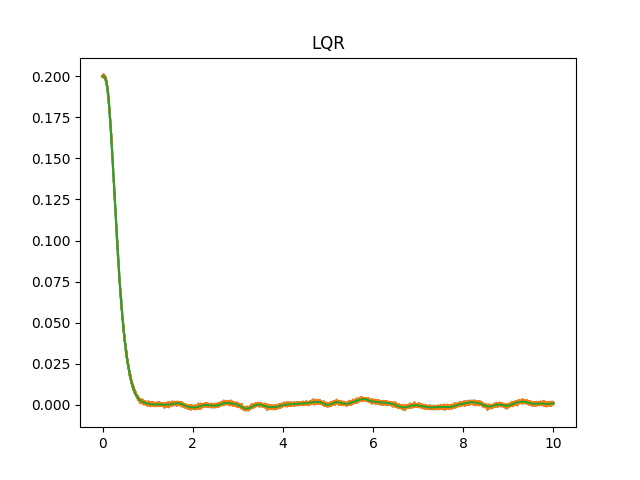
\includegraphics[scale=1]{fig/LQR_regulation.png} 
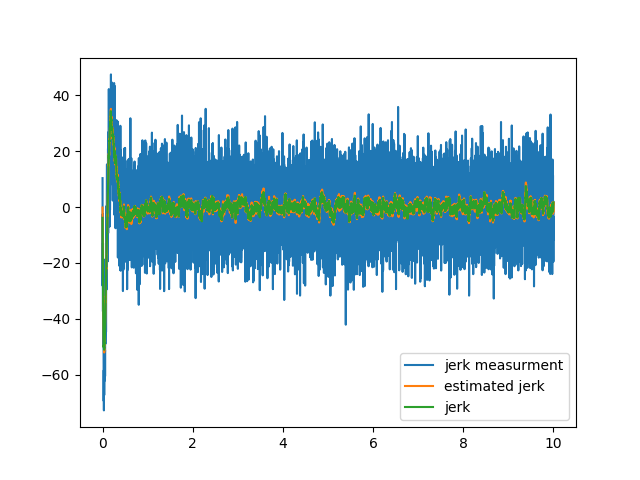
\includegraphics[scale=1]{fig/LQR_jerk_estimation.png}
\caption{LQR with Pole=[-10, -11, -12, -13]}
\label{Tux}
\end{figure}


\end{document}